\section{Lance Architecture}
\label{lance-sec-architecture}

\begin{figure}[t]
\begin{center}
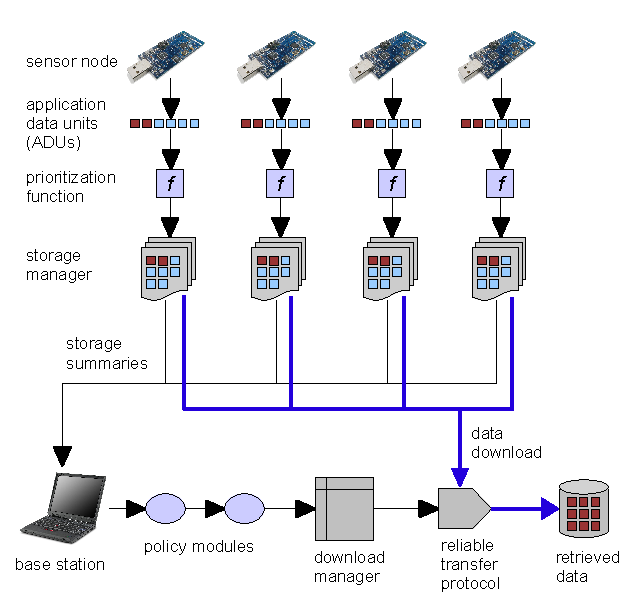
\includegraphics[width=0.8\hsize]{./4-lance/figs/architecture.pdf}
\end{center}

\caption{\textbf{The Lance system architecture.} The summarization portions
are provided by the application; all other components are generic.}

\label{lance-fig-architecture}
\end{figure}

This section describes the Lance architecture, introducing a formal problem
definition, design principles, and major system components.

\subsection{Problem Definition}
\label{lance-sec-problem-definition}

In Lance, the network consists of a set of sensor nodes that continuously
sample and store sensor data into \textit{application data units (ADUs)},
which are the unit of data storage and retrieval. Each unique ADU $a_i$
consists of a tuple $\{ i, n_i, t_i, d_i, v_i, \bar{c}_i \}$, where:

\begin{itemize}

\item $i$ is a unique ADU identifier,

\item $n_i$ is the node storing the ADU,

\item $t_i$ is a timestamp,

\item $d_i$ is the raw sensor data,

\item $v_i$ is a utility value assigned to this ADU, and

\item $\bar{c}_i$ is a the cost vector associated with this ADU.

\end{itemize}

We assume that ADUs are of uniform size and that nodes have sufficient flash
storage to buffer collected signals, so an ADU is only evicted from a node's
flash once it has been downloaded. We define the \textit{universe} $U$ as the
set of all ADUs sampled by the network over time.

Every ADU is assigned an application-specific \textit{value} $v_i$ that
represents the application's intrinsic ``utility'' for the data contained
within the ADU. The value assignment begins by the sensor nodes computing
summaries, and completes on the base station with the application and policy
modules transforming the summary into a value. This process is described
below. We make no assumptions about how ADU values are assigned. The value
could be a function of the data itself, the time the data was acquired, which
node sampled the data, data being sampled by other nodes, and so forth.
Lance provides a flexible infrastructure for applications to define their own
value functions through policy modules.

Each ADU has an associated cost $\bar{c}_i$ that represents the energy
requirement to download the ADU from the network. $\bar{c}_i$ is a vector $\{
c_i^1, c_i^2, \ldots, c_i^n \}$ where $c_i^j$ represents the estimated energy
expenditure of node $j$ when ADU $i$ is retrieved. $\bar{c}_i$ is computed by
Lance at the base station usins its knowledge of the routing topology and
link costs. The key idea is that we explicitly model both the energy cost for
downloading the ADU from its ``host'' node $n_i$ and the energy cost for each
node along the routing path from $n_i$ to the base station which must forward
packets during the transfer. In addition, we also model the energy cost to
nodes that overhear transmissions by nodes participating in the transfer.
This energy cost on intermediate nodes is non-negligible, since reliable
transfer protocols involve a potentially large number of retransmission.
However, the overhearing cost is typically small, since modern low-power MAC
protocols quickly return to sleep when overhearing transmissions to another
node. The cost vector $\bar{c}_i$ therefore depends on the network topology.

We assume that each node has a battery with a fixed capacity of $C$ joules,
and no energy harvesting is performed in the field. Without loss of
generality, let us assume that $C$ is identical for all nodes in the network
and is known \textit{a priori}. We define the \textit{lifetime target} $L$
as the desired lifetime of each node in the network. To meet the lifetime
target, nodes should strive to consume no more than $C/L$ joules per unit
time on average; we call this the \textit{discharge rate} of the node.

The high-level goal of Lance is to download the set of ADUs that maximizes
the total value, subject to the lifetime target. Abstractly, we define an
\textit{epoch duration} $\Delta$. Over each epoch, the energy consumption of
each node must be less than the discharge rate, that is, $\sum_i \sum_j c_i^j
\leq \Delta \times C/L$. Determining the optimal set of ADUs to download can
be determined by solving a multidimensional knapsack problem in which each
ADU represents an item to place in the knapsack with value $v_i$ and cost
$\bar{c}_i$. The knapsack has $N$ dimensions (where $N$ is the number of
nodes in the network), each of size $\Delta \times C/L$ representing the
energy availability over an epoch.

Calculating the optimal knapsack solution requires \textit{a priori}
knowledge of all ADUs generated by the network over time. Because we assume
no such knowledge, our system uses an online, heuristic algorithm to
approximate the optimal solution. We discuss and evaluate several different
approaches, presenting results with respect to the optimal offline solution.

Intermediate points exist, however, between our assumption of no prior
knowledge and the complete knowledge required by the offline optimal
solution. We might imagine that estimates of the distribution of ADU values
could be computed before deployment (using datasets expected to have similar
properties) or in the field either during a calibration or continuously as
the system collects data. The Lance architecture can support applications
that would benefit from these approaches using the policy modules described
in the next section, but we have not included them in the base architecture
in order to support other applications for which they are not appropriate.

\subsection{Design Principles}

Before describing Lance in detail, we first outline several principles
that guide its design.

\begin{enumerate}

\item \textbf{Decouple mechanism from policy.} We wish to make it easy to
adapt Lance to different application domains by providing a simple set of
underlying mechanisms for weighing cost and data value that can be tailored
for different end-user goals. These core mechanisms should not be tied to any
interpretation of the data stored in an ADU. This approach leads to a clean
separation of concerns between Lance's resource management layer and the
higher-level policies informing its operation.

\item \textbf{Simplicity through centralized control.} In a field deployment
setting, it is highly desirable for the sensor network to be as simple as
possible, to prevent failures or unexpected behavior due to bugs. Past
deployment experiences taught us (and others) that introducing complex
dynamics within the network can lead to a system that is difficult to
understand, debug, or fix in the field. To maximize the chances of a
successful deployment, Lance places most of the control logic at the base
station, treating sensor nodes as slave devices. This principle makes it easy
to change the behavior of the network at the base station and allows nodes to
fail independently without affecting the rest of the system. Conventional
replication and failover techniques can be used to bolster the reliability of
the base station itself.

\item \textbf{Low cost for maintenance traffic.} Given limited node energy,
we wish to reserve as much capacity as possible to support data collection.
This implies that the system should strive to limit control messages between
the base station and the sensor nodes, as well as internal traffic within the
network, as transmitting packets unnecessarily consumes valuable energy.
This is somewhat at odds with the need for central control, as the latter
could require extensive coordination between sensor nodes and the base
station; we wish to strike a good balance between these two conflicting
goals.

\end{enumerate}

\subsection{System Overview}

Figure~\ref{lance-fig-architecture} provides an overview of the Lance
architecture. Sensor nodes sample sensor data, storing the data to local
flash storage. Each application data unit (ADU) consists of some amount of
raw sensor data, a unique \textit{ADU identifier}, and a \textit{timestamp}
indicating the time that the first sample in the ADU was sampled. ADU
timestamps can either be based on local clocks at each node or tied to a
global timebase using a time synchronization protocol such as
FTSP~\cite{ftsp}. The size of an ADU should be chosen to balance the
granularity of data storage and download with the overhead for maintaining
per-ADU metadata. In the applications we have studied, an ADU stores several
seconds or minutes of sensor data, not an individual sample. ADUs are stored
locally in flash, which is treated as a circular buffer.

Ideally, nodes would be able to compute the value $v_i$ of an ADU locally, as
the data is sampled. However, since the value might depend on factors other
than the ADU's data, such as data computed at other nodes, Lance assigns
values $v_i$ at the base station, based on global knowledge of the state of
the network. However, this requires nodes to communicate some low-bandwidth
information on the ADU contents to the base station. For this purpose, each
node applies an application-supplied \textit{summarization function},
computing a concise summary, $s_i$, of the contents of the ADU as it is
sampled. Nodes periodically send \textit{ADU summary} messages to the base
station, providing information about the ADUs they have sampled, their
summaries, timestamps, and other metadata. As a special case, if a node is
able to assign the ADU's initial value directly, this is used as the summary.

The Lance \textit{controller} receives ADU summaries from the network. The
controller also estimates the download cost $\bar{c}_i$ for each ADU, based
on information about network topology as well as a model of energy
consumption for download operations. The ADU summaries and cost are passed
through a series of \textit{policy modules}, which provide
application-specific logic to assign the value $v_i$ to each ADU. The
resulting values are passed to the Lance \textit{download manager} which is
responsible for performing downloads, using a reliable data-collection
protocol, such as Flush~\cite{flush-sensys07}.

\subsection{Two-Tiered Value Assignment}

Dividing the overall value computation into two components --- local
summarization running on each node and global application value assignment
and policy modules running at the base station --- attempts to reap the
benefits of global control while minimizing the costs. Fully accurate global
value assignment requires downloading all data to the base station and
reduces to full signal collection, which we have already argued is
infeasible.

Purely local assignment, where nodes each determine what data to send to the
base station, is possible but also problematic. Due to sensor and node
differences we assume that nodes will not be able to determine what data is
truly ``interesting'' without additional coordination. The highest-value ADU
on one node may have a value below all ADUs on another, if the first has a
poor sensor or the second is located near more interesting events. We could
imagine working around this by having nodes send information about their
local value distributions to some central location and then have information
returned about how interesting their data is relative to others. This is
similar in many ways to what we accomplish with Lance.

The purely local approach also cannot easily support the cross-node
visibility that Lance applications and policy modules benefit from due to
their position at the base station. Of course, this information could be
distributed throughout the network to allow each node to mimic the base
station's behavior, but the overhead of such global state sharing would
likely be higher than the cost of aggregating the summaries in Lance.

Finally, the ability to easily change the network's operation without
reprogramming nodes was another feature that argued for our two-tiered
approach. Our initial deployment experiences described in the previous
chapter left us wary of pushing too much complexity onto the nodes
themselves.

\subsection{Summarization Functions}

Lance computes ADU values using two application-provided components. The
first is the summarization function, described above. The second component is
a chain of \textit{policy modules} executed at the base station which, by
modifying the value for each ADU, can implement a range of
application-specific policies. Since the base station receives ADU summaries
from every node, the policy modules can use global information not available
to individual nodes to make informed bandwidth and energy allocation
decisions.

Lance places two constraints on the summarization function. First, we require
that the summary be small (typically a few bytes) to limit the overhead for
storing and transmitting these values. Second, the function must be able to
run efficiently on the sensor node as ADUs are being sampled. Otherwise, the
exact form of the function is entirely application-specific.

As a concrete example, consider a network for downloading seismic events from
an earthquake zone. One commonly-used measure of overall seismicity during a
time period is the Real-Time Seismic Amplitude Measurement
(RSAM)~\cite{rsam}, which computes the average amplitude of a seismic signal
over some time window (typically 1~to~10~minutes). This function is simple to
compute and reduces a complex seismic waveform to a single scalar value, with
higher values indicating greater seismic activity.

Another form of summarization is an event detector, which would produce a
nonzero value whenever an event of interest is contained within the ADU; the
summary might also represent the strength or confidence of the event
detection. For example, an acoustic animal tracking
system~\cite{girod-ipsn07} or countersniper localization
system~\cite{shooter-localization} might use a simple trigger-based
summarization function, indicating the detection of a marmot call or gunshot
in the ADU.

\subsection{Cost Estimation}
\label{lance-subsec-costestimation}

Lance estimates the download energy cost vector $\bar{c}_i$ for each ADU
sampled by the network. We assume that nodes are organized into a spanning
tree topology rooted at the base station. The cost is a function of many
factors, including the reliable transport protocol, each node's position in
the routing tree, radio link quality characteristics, and the MAC protocol.

Given the complex dynamics that can arise during a sensor network's
operation, we opt to use a simple conservative estimate of the energy cost to
download an ADU from a node. Our approach is based on an empirical model that
captures three primitive energy costs involved in downloading an ADU. The
first, $E_d$, represents the energy used to download an ADU from a given
node, which includes the energy cost for reading data from flash and sending
multiple radio packets (including any retransmissions) to the next hop in the
routing tree. The second, $E_r$, represents the energy cost at intermediate
nodes to forward messages during the ADU transfer. The third, $E_o$,
represents the energy cost to nodes that overhear transmissions during a
transfer. For simplicity, we assume ADUs of fixed size and compute $E_d$,
$E_r$, and $E_o$ based on the time necessary to download an ADU from the
target node.

Using this simple model, we set the elements of the cost vector $\bar{c}_i$
as follows. $c_i^n = E_d$ for the node $n$ hosting the ADU, and $c_i^m = E_r$
for nodes $m$ along the routing path from $n$ to the base station. We set
$c_i^o = E_o$ for nodes that are assumed to be within one radio hop of any of
the nodes involved in the transfer. Estimating $\bar{c}_i$ therefore requires
knowledge of the current routing topology. This information is readily
available: the periodic summary messages, sent to the base station by every
node, include the node's radio neighbors and parent in the routing tree. Cost
vectors can be easily recomputed whenever the routing topology changes.

To ensure that all nodes meet the lifetime target $L$, Lance models the
energy availability at each node using a token bucket with depth $D$ and fill
rate $C/L$, corresponding to the mean discharge rate. $D$ is determined by
the target lifetime $L$, the battery capacity $B$ and the background drain
rate $R$. In general, $D = B - L*R$, so $D$ represents the energy remaining
after the node reserves enough to ensure it can meet its target lifetime at
the background level.

\subsection{Lance Optimizer}
\label{lance-subsec-optimizer}

The Lance optimizer is responsible for scheduling ADUs for download, based on
knowledge of the set of ADUs currently stored by the network, their
associated values, and the costs of downloading them. ADU download itself is
accomplished using a reliable transfer protocol (such as Fetch or
Flush~\cite{flush-sensys07}). In our design, Lance attempts to download a
single ADU at a time, in order to prevent network congestion, although it may
be possible to download multiple ADUs simultaneously, depending on the
network topology. A download completes either when the entire ADU has been
received or a timeout occurs.

Lance's optimization process attempts to maximize the value of the ADUs
retrieved while adhering to the lifetime target $L$. In essence, we seek a
greedy heuristic approximation of the multidimensional knapsack solution that
would be used by an oracle with complete knowledge of the ADUs sampled by the
network over all time. The optimizer first excludes ADUs that would involve
nodes without enough energy to perform a download. That is, if the token
bucket for a given node $m$ has $E(m)$ joules, ADUs for which $E(m) < c_i^m$
are excluded from consideration. Note that as the bucket fills, the ADU may
become available for download at a later time. We call these ADUs
\textit{infeasible}, and the remaining \textit{feasible}.

To determine the next ADU to download, the optimizer considers the value
$v_i$ of each feasible ADU and the its associated cost $\bar{c}_i$. We
consider three \textit{scoring functions} that assign a download score to
each feasible ADU; the ADU with the highest download score is downloaded
next. In the case of ties, an arbitrary ADU is chosen.

The first scoring function, \textit{value-only}, simply downloads the
feasible ADU with the highest value $v_i$. Note that \textit{value-only} will
meet the network's lifetime target (since only feasible ADUs are considered)
but does not rank ADUs according to cost. The second scoring function,
\textit{cost-total}, assigns the score $\hat{v}_i$ by scaling the value of
the ADU by its total cost: $\hat{v}_i = v_i / \sum_j c_i^j$. The feasible ADU
with the highest score is then downloaded from the network. This approach
penalizes ADUs stored deep in the routing tree, which have a higher overall
cost than those located near the base station.

The third scoring function, \textit{cost-bottleneck}, scales the ADU value
$v_i$ by the cost to the node that is an energy bottleneck for downloading
this ADU. That is, let $b$ represent the node with the minimum value of
$E(b)$ such that $c_i^b > 0$. \textit{cost-bottleneck} sets the score
$\hat{v}_i = v_i / c_i^b$. The intuition behind this scoring function is that
the most energy-constrained node should be considered when scoring ADUs for
download. We evaluate all three scoring functions in this chapter and show
that they yield rather different results in terms of spatial distribution and
energy efficiency.
